\section{The Heugh transorm}\label{ssec:heugh_tf}
The Hough transform was first introduced by \cite{10.1145/361237.361242} for the application of detecting lines in an image. Reducing this problem to finding lines in a set of $N$ points $(x_i, y_i)\in \Omega$ where $x_i\in [0..X]$, $y_i\in [0..Y]$ and $i\in [0..N]$. $X$ is the size in the first x-dimension and $Y$ the size in the second y-dimension of the image.\\
Assuming each point lies on a line, transferring each point to the latent space of lines defined by the \emph{normal parameterization} of a line. As shown in figure \ref{fig:norm_line} this is defined by the angle $\theta$ of the lines normal and its algebraic distance $\rho$ from the origin.\\

\begin{figure}[ht!]
	\centering
	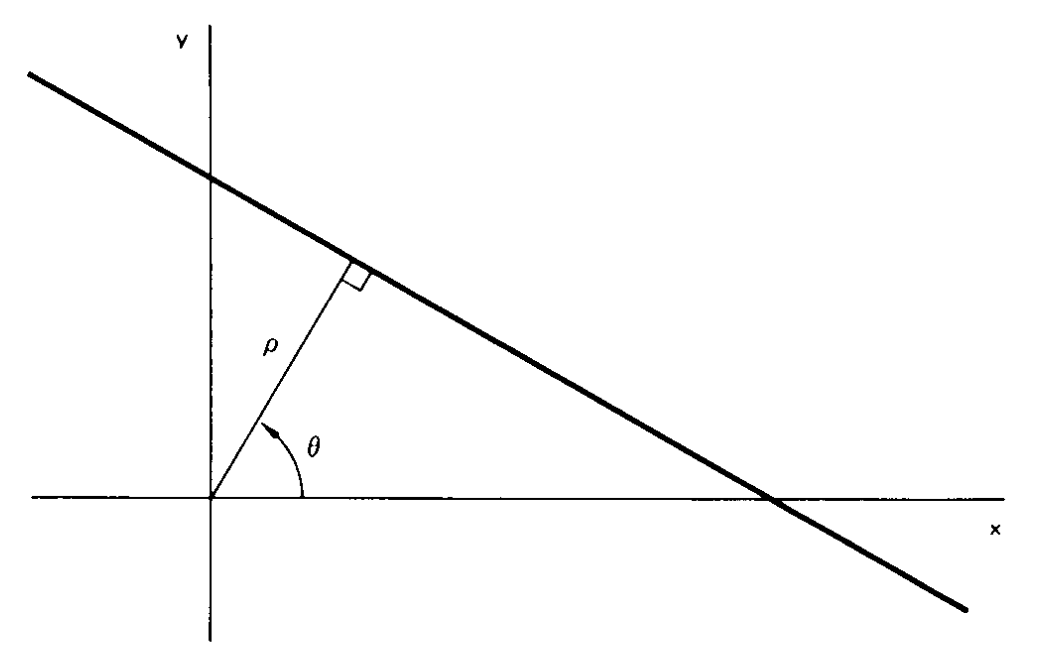
\includegraphics[width=.5\textwidth]{figures/heugh_line.png}
	\caption{latent variables of a line \cite{10.1145/361237.361242}}
	\label{fig:norm_line}
\end{figure}

Transforming all points in $\Omega$ to sinusoidals in the $\theta$-$\rho$ plane yields
\begin{align}
	\rho_i(\theta) = x_i \cos \theta + y_i \sin \theta \text{, \hspace{8mm} \forall $i\in [0..N]$}
\end{align}
One property of this point to curve transformation is, that a intersection of two or more of those functions means that there is a line in the image plane, going through all points the functionals correspond to.\\
Therefore lines are found by discretizing the $\theta$-$\rho$ plane and counting in each cell the intersections of functions $\rho_i(\theta)$ going through that cell.\\
Thresholding leaves only the cells with a count of intersections higher than the thresholding parameter and each of those cells can be transformed to a line in the image space.\\
This idea can be extended to the detection of circles resulting in the Circle Heugh transform (CHT). A parametric representation for a circle in the x-y plane is given by 
\begin{align}
	c^2 = (x-a)^2 + (y-b)^2
\end{align}
and a point $(x_i, y_i)$ in the image place can be transformed to a surface in the $a$-$b$-$c$ parameter space.

\begin{align}
c_i^2(a, b) = (x_i-a)^2 + (y_i-b)^2
\end{align}

this surface correponds to a right circular cone. Again intersections of multiple functionals $c_i(a, b)^2$ means that the corresponding points in the image plane correspond to the circle defined by the intersection point in the $a$-$b$-$c$ parameter space. The same procedure of discretizing and counting as for the line detection method results in the CHT as defined in \cite{10.1145/361237.361242}.
